\documentclass[abstract=on,10pt,a4paper,bibliography=totocnumbered]{article}
\usepackage[paper=a4paper,left=35mm,right=35mm,top=25mm,bottom=30mm]{geometry}
\usepackage[doublespacing]{setspace}
\usepackage[english]{babel}
\usepackage[utf8]{inputenc}
\usepackage[round]{natbib}
\usepackage{amsmath}
\usepackage{colortbl}
\usepackage{amsfonts}
\usepackage{amssymb}
\usepackage{gensymb}
\usepackage{graphicx}
\usepackage{tikz}
\usepackage{enumerate}
\usepackage{enumitem}
\usepackage{subcaption}
\usepackage{booktabs}
\usepackage[hidelinks]{hyperref}
\usepackage[nameinlink]{cleveref}
% \usepackage{lineno}
\usepackage{multirow}
\usepackage{arydshln}
\usepackage[flushleft]{threeparttable}
\usepackage[nomarkers, nolists]{endfloat}
\usepackage[colorinlistoftodos]{todonotes}
\usepackage{scalerel}
\usepackage{tikz}
\usetikzlibrary{svg.path}

%------------------------------------------------------------------------------
%	Some Styling
%------------------------------------------------------------------------------
% Creating some TikZ styles
\tikzset{
  nonterminal/.style = {rectangle
    , minimum size = 6mm
    , very thick
    , draw = black!
  }
}

% Changing the style of captions in figures etc.
\captionsetup{labelfont=bf, format=plain, font=small}

% Change how equations are referenced
\renewcommand{\theequation}{Equation \arabic{equation}}%

% To be able to put an ORCID
\definecolor{orcidlogocol}{HTML}{A6CE39}
\tikzset{
  orcidlogo/.pic={
    \fill[orcidlogocol] svg{M256,128c0,70.7-57.3,128-128,128C57.3,256,0,198.7,0,128C0,57.3,57.3,0,128,0C198.7,0,256,57.3,256,128z};
    \fill[white] svg{M86.3,186.2H70.9V79.1h15.4v48.4V186.2z}
                 svg{M108.9,79.1h41.6c39.6,0,57,28.3,57,53.6c0,27.5-21.5,53.6-56.8,53.6h-41.8V79.1z M124.3,172.4h24.5c34.9,0,42.9-26.5,42.9-39.7c0-21.5-13.7-39.7-43.7-39.7h-23.7V172.4z}
                 svg{M88.7,56.8c0,5.5-4.5,10.1-10.1,10.1c-5.6,0-10.1-4.6-10.1-10.1c0-5.6,4.5-10.1,10.1-10.1C84.2,46.7,88.7,51.3,88.7,56.8z};
  }
}
\newcommand\orcid[1]{\href{https://orcid.org/#1}{\mbox{\scalerel*{

\begin{tikzpicture}[yscale=-1,transform shape]
  \pic{orcidlogo};
\end{tikzpicture}
}{|}}}}

%------------------------------------------------------------------------------
%	Titlepage: Header
%------------------------------------------------------------------------------
\title{Flooding of the Okavango Delta influences Connectivity for Dispersing
African Wild Dogs}

% List of Authors
\author{
  David D. Hofmann\textsuperscript{1,2,\S} \orcid{0000-0003-3477-4365} \and
  Gabriele Cozzi\textsuperscript{1,2} \orcid{0000-0002-1744-1940} \and
  John W. McNutt\textsuperscript{2} \and
  Arpat Ozgul\textsuperscript{1} \orcid{0000-0001-7477-2642} \and
  Dominik M. Behr\textsuperscript{1,2} \orcid{0000-0001-7378-8538}
}

% Reduce spacing between authors
\makeatletter
\def\and{%
  \end{tabular}%
  \hskip -0.5em \@plus.17fil\relax
  \begin{tabular}[t]{c}}
\makeatother

% Current Date
% \date{\today}

% And here the masterpiece begins
\begin{document}

% Change page numbering
\pagenumbering{gobble}

% Required to be able to cite
\bibliographystyle{apalike}

% Create Titlepage
\maketitle

%------------------------------------------------------------------------------
%	Titlepage: Additional Info
%------------------------------------------------------------------------------
\begin{flushleft}

\vspace{0.5cm}

\textsuperscript{1} Department of Evolutionary Biology and Environmental
Studies, University of Zurich, Winterthurerstarsse 190, 8057 Zurich,
Switzerland.

\textsuperscript{2} Botswana Predator Conservation Program, Private Bag 13,
Maun, Botswana.

\textsuperscript{\S} Corresponding author (david.hofmann2@uzh.ch)

\vspace{4cm}

\textbf{Running Title:} None

\vspace{0.5cm}

\textbf{Keywords:} Seasonal Flooding of the Okavango Delta and its Consequences
for African Wild Dog Connectivity

\end{flushleft}

%------------------------------------------------------------------------------
%	Abstract
%------------------------------------------------------------------------------
\newpage
\begin{abstract}
Many ecosystems experience drastic changes in environmental conditions due to
seasonality. While such seasonal changes may drastically alter connectivity for
endangered species, most studies represent the environment by a static set of
spatial layers, thus ignoring seasonal changes. Here, we address this
shortcoming and employ individual-based simulations to investigate how seasonal
flooding of the Okavango delta influences connectivity for dispersing African
wild dogs (\textit{Lycaon pictus}). Our results show that the Okavango delta
poses a substantial dispersal barrier when the flood is at maximum extent, yet
that viable dispersal corridors exist when the flood is at a minimum level.
Despite a better understanding of the conservation needs for African wild dogs,
our study also provides evidence that incorporating seasonality in studies of
connectivity is imperative to more accurately predict dispersal ability of
endangered species.
\end{abstract}

%------------------------------------------------------------------------------
%	Main Text
%------------------------------------------------------------------------------
\newpage

\onehalfspacing
\tableofcontents
\doublespacing

% Change page numbering
\newpage
\pagenumbering{arabic}

% Create linenumbers
% \linenumbers

\section{Introduction}
Hello, I'm an introduction.

\section{Methods}

\subsection{Study Area}
As depicted in \Cref{StudyArea}, the study area encomassed ...

\begin{figure}
  \begin{center}
  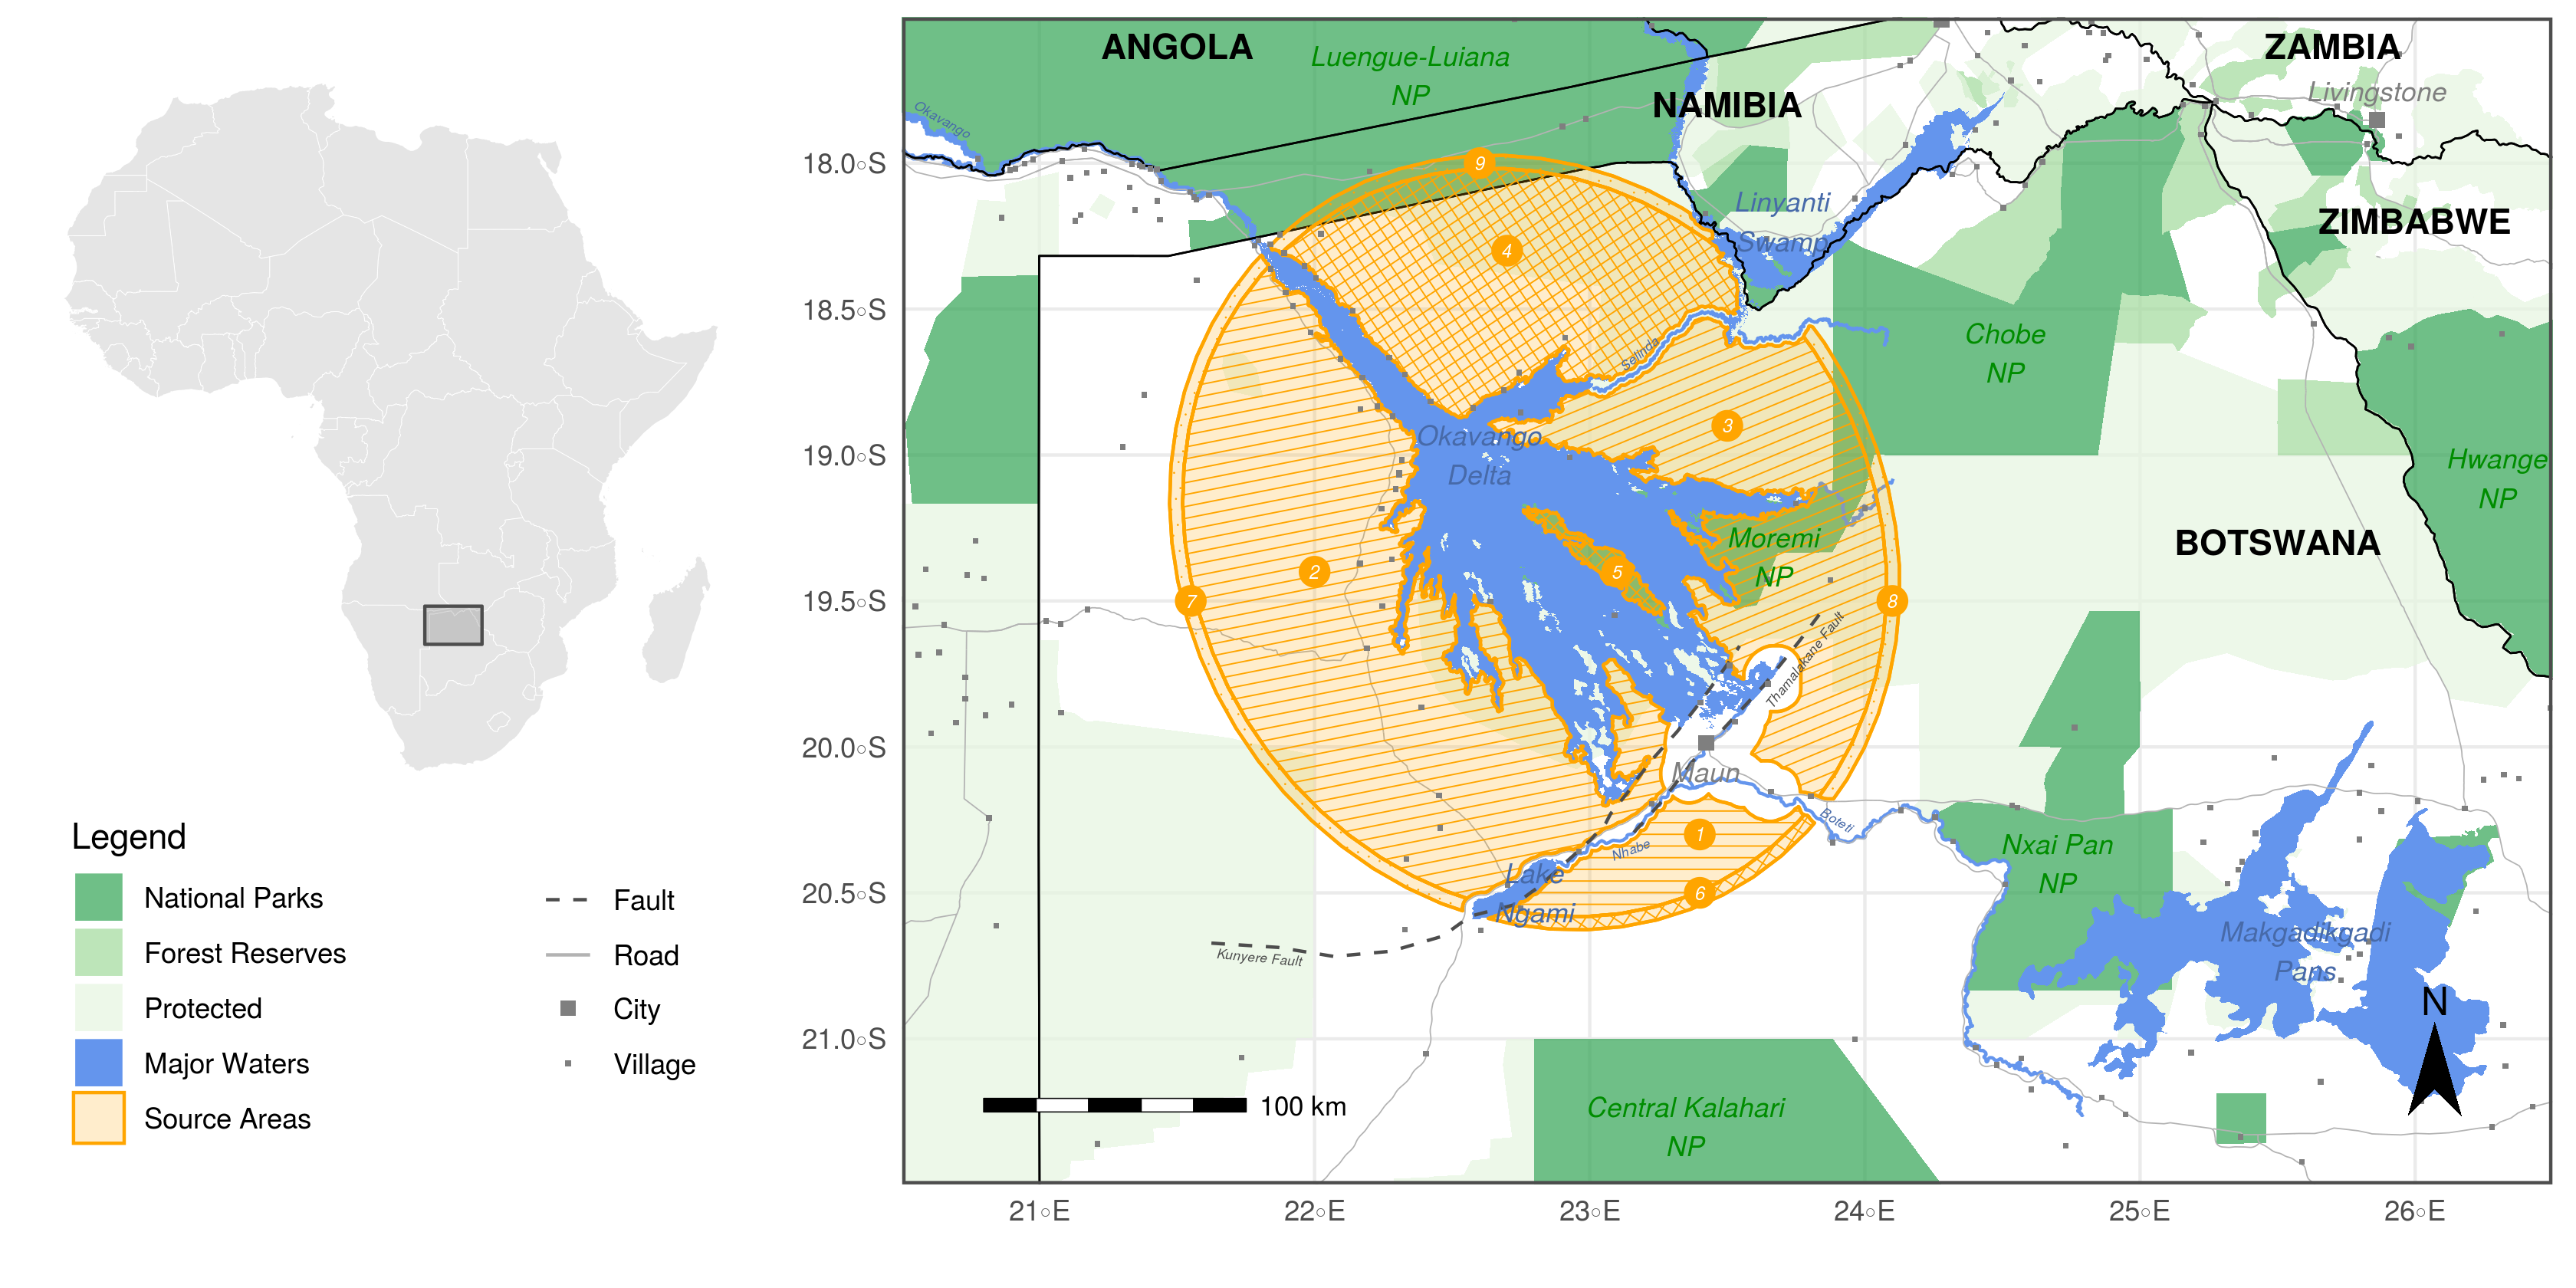
\includegraphics[width = \textwidth]{99_StudyArea.png}
  \caption{Study area across which we simulated dispersal events. Virtual
  dispersers were released at random locations within the orange source areas.}
  \label{StudyArea}
  \end{center}
\end{figure}

\subsection{Flood}
In order to generate spatial layers that depict the flood extent at different
points in time, we ... \Cref{FloodExtent}.

\begin{figure}
  \begin{center}
  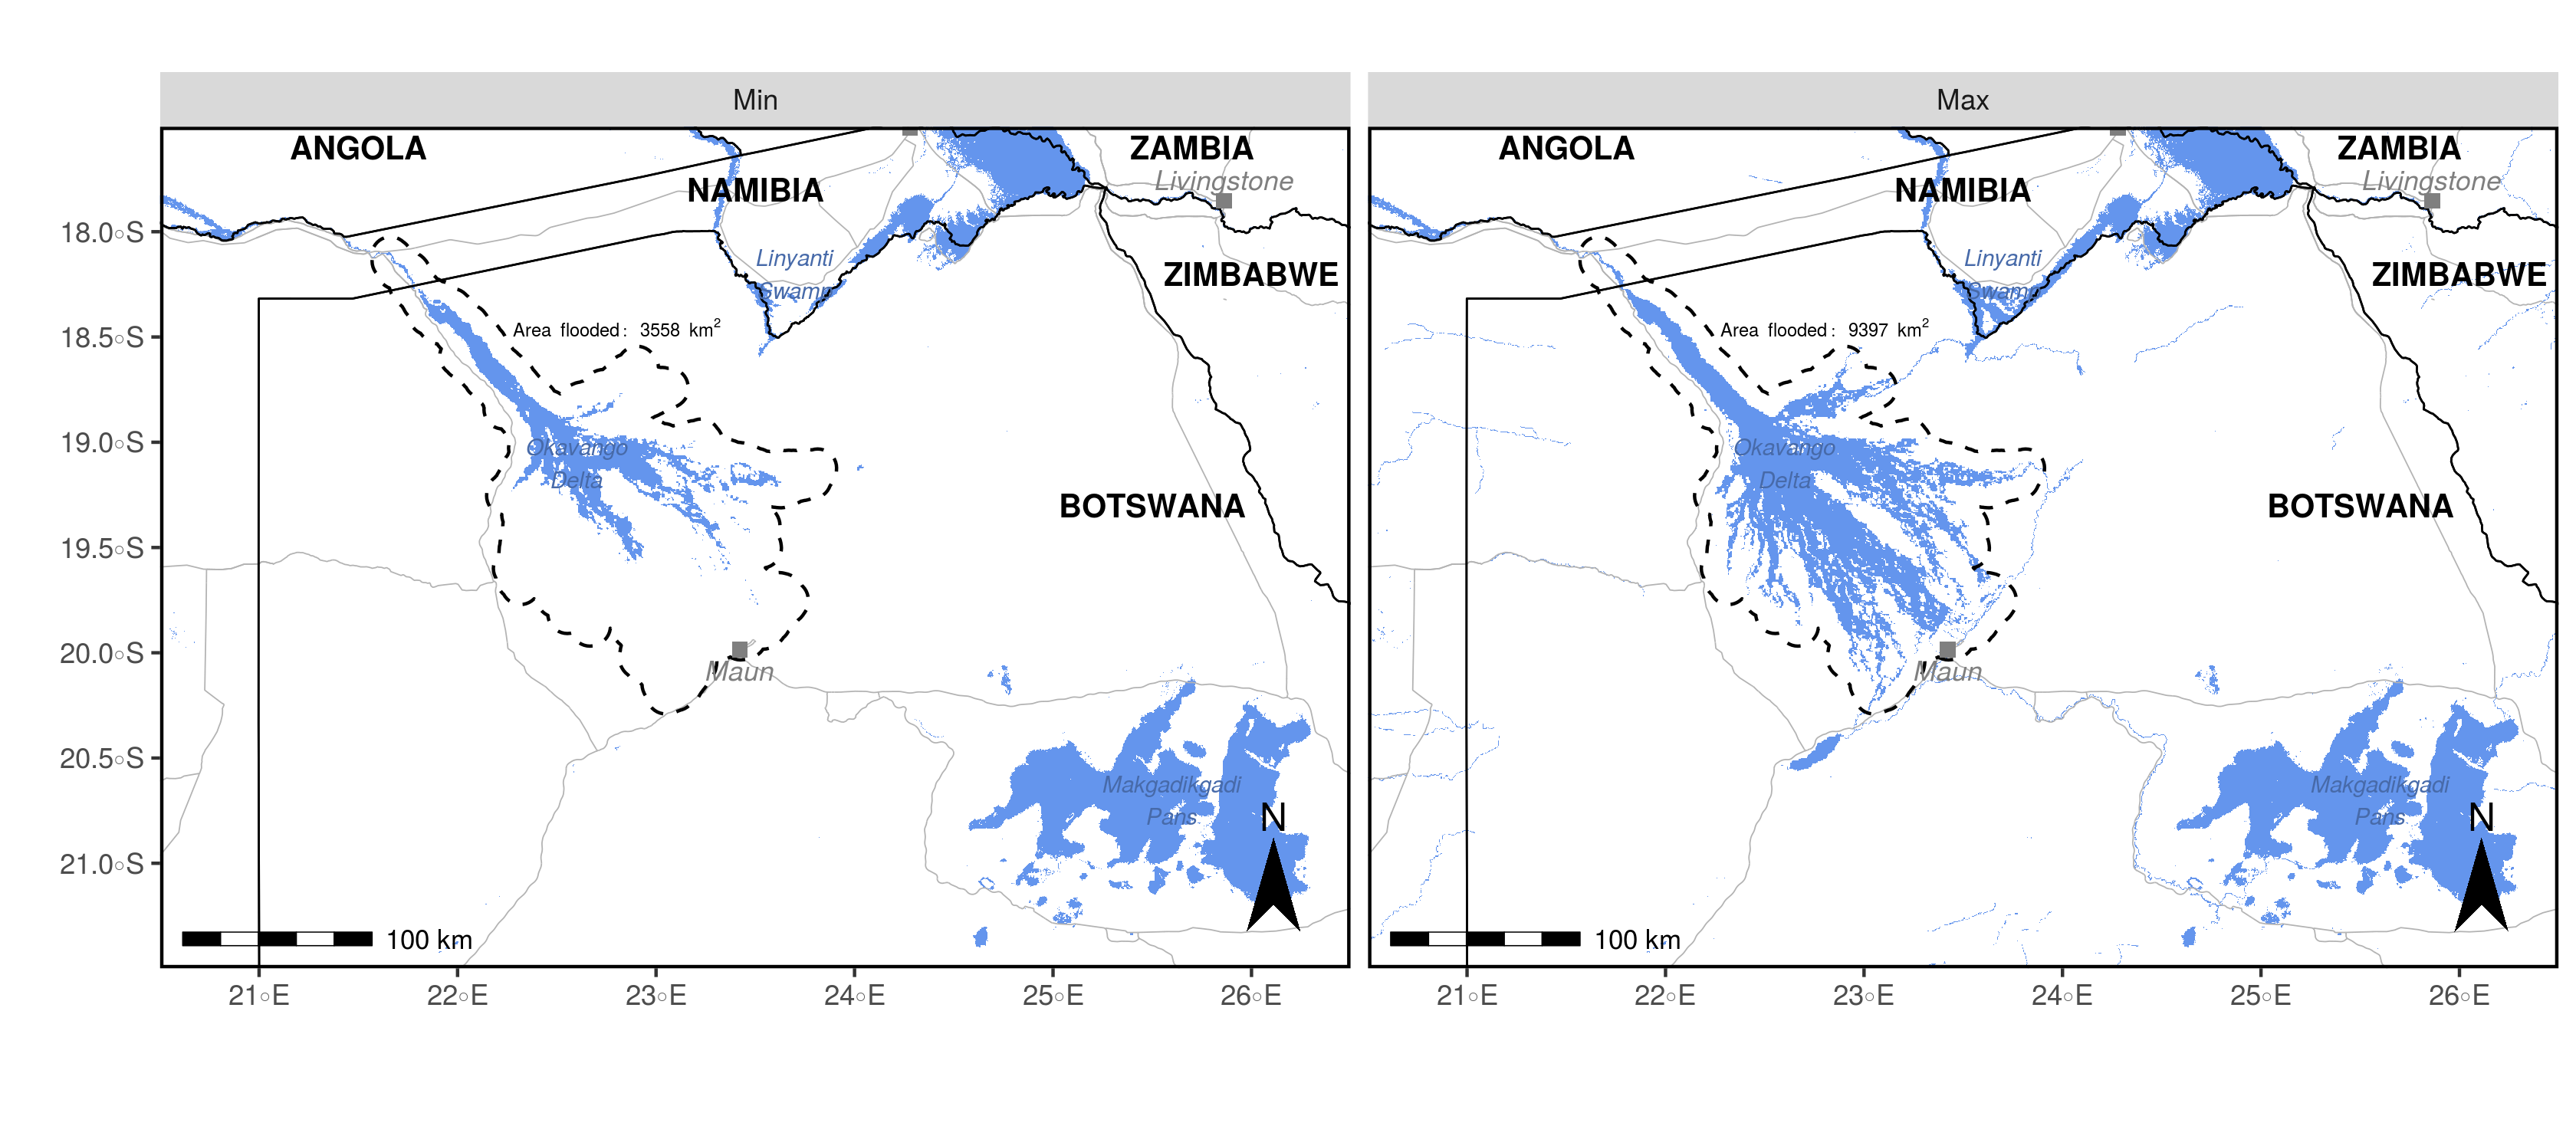
\includegraphics[width = \textwidth]{99_FloodExtent.png}
  \caption{}
  \label{FloodExtent}
  \end{center}
\end{figure}


\section{Authors' Contributions}
D.D.H., D.M.B., A.O. and G.C. conceived the study and designed methodology;
D.M.B., G.C., and J.W.M. collected the data; D.D.H. and D.M.B. analysed the
data; G.C. and A.O. assisted with modeling; D.D.H., D.M.B., and G.C. wrote the
first draft of the manuscript and all authors contributed to the drafts at
several stages and gave final approval for publication.

\section{Data Availability}
GPS movement data of dispersing wild dogs is available on dryad
\citep{Hofmann.2021b}. Access to R-scripts that exemplify the application of the
proposed approach using simulated data are provided through Github
(\url{https://github.com/DavidDHofmann/DispersalSimulation}). In addition, all
codes required to reproduce the African wild dog case study will be made
available through an online repository at the time of publication.

\section{Acknowledgements}
We thank the Ministry of Environment and Tourism of Botswana for granting
permission to conduct this research. We thank C. Botes, I. Clavadetscher, and G.
Camenisch for assisting with wild dog immobilizations. We also thank B. Abrahms
for sharing her data of three dispersing wild dogs. Furthermore, we would like
to thank Johannes Signer for assisting with the simulation algorithm. This study
was funded by Albert-Heim Foundation, Basler Stiftung für Biologische Forschung,
Claraz Foundation, Idea Wild, Jacot Foundation, National Geographic Society,
Parrotia Stiftung, Stiftung Temperatio, Wilderness Wildlife Trust Foundation,
Forschungkredit der Universität Zürich, and a Swiss National Science Foundation
Grant (31003A\_182286) to A. Ozgul.

\newpage
\begingroup
\singlespacing
\bibliography{Literatur}
\endgroup

\end{document}
